\let\negmedspace\undefined
\let\negthickspace\undefined
\documentclass[journal]{IEEEtran}
\usepackage[a5paper, margin=10mm, onecolumn]{geometry}
%\usepackage{lmodern} % Ensure lmodern is loaded for pdflatex
\usepackage{tfrupee} % Include tfrupee package

\setlength{\headheight}{1cm} % Set the height of the header box
\setlength{\headsep}{0mm}     % Set the distance between the header box and the top of the text

\usepackage{gvv-book}
\usepackage{gvv}
\usepackage{cite}
\usepackage{amsmath,amssymb,amsfonts,amsthm}
\usepackage{algorithmic}
\usepackage{graphicx}
\usepackage{textcomp}
\usepackage{xcolor}
\usepackage{txfonts}
\usepackage{listings}
\usepackage{enumitem}
\usepackage{mathtools}
\usepackage{gensymb}
\usepackage{comment}
\usepackage[breaklinks=true]{hyperref}
\usepackage{tkz-euclide} 
\usepackage{listings}
                                         
\def\inputGnumericTable{}                                 
\usepackage[latin1]{inputenc}                                
\usepackage{color}                                            
\usepackage{array}                                            
\usepackage{longtable}                                       
\usepackage{calc}                                             
\usepackage{multirow}                                         
\usepackage{hhline}                                           
\usepackage{ifthen}                                           
\usepackage{lscape}
\begin{document}


\bibliographystyle{IEEEtran}

\title{5.8.19}
\author{EE25BTECH11021 - Dhanush sagar}
% \maketitle
% \newpage
% \bigskip
\maketitle \vspace{-1cm}
\renewcommand{\thefigure}{\theenumi}
\renewcommand{\thetable}{\theenumi}
\setlength{\intextsep}{10pt} % Space between text and floats

\
\numberwithin{figure}{enumi}
\renewcommand{\thetable}{\theenumi}

\textbf{Question:}  \\
Let $a, b, c$ be real numbers. Consider the following system of equations in $x, y, z$:
\begin{align*}
\frac{x^2}{a^2} + \frac{y^2}{b^2} - \frac{z^2}{c^2} &= 1, \\
\frac{x^2}{a^2} - \frac{y^2}{b^2} + \frac{z^2}{c^2} &= 1, \\
-\frac{x^2}{a^2} + \frac{y^2}{b^2} + \frac{z^2}{c^2} &= 1.
\end{align*}
The system has:
\begin{enumerate}
    \item no solution
    \item unique solution
    \item infinitely many solutions
    \item finitely many solutions
\end{enumerate}


\begin{solution}
Let
\begin{align}
A &= \frac{x^2}{a^2}, \\
B &= \frac{y^2}{b^2}, \\
C &= \frac{z^2}{c^2}.
\end{align}

Then the system becomes
\begin{align}
A + B - C &= 1, \\
A - B + C &= 1, \\
- A + B + C &= 1.
\end{align}

The augmented matrix is
\begin{align}
\myvec{1 & 1 & -1 & 1 \\ 1 & -1 & 1 & 1 \\ -1 & 1 & 1 & 1}
&\xrightarrow{R_2 \to R_2 - R_1}
\myvec{1 & 1 & -1 & 1 \\ 0 & -2 & 2 & 0 \\ -1 & 1 & 1 & 1} 
\xrightarrow{R_3 \to R_3 + R_1}
\myvec{1 & 1 & -1 & 1 \\ 0 & -2 & 2 & 0 \\ 0 & 2 & 0 & 2} \notag\\
&\xrightarrow{R_3 \to R_3 + R_2}
\myvec{1 & 1 & -1 & 1 \\ 0 & -2 & 2 & 0 \\ 0 & 0 & 2 & 2} 
\xrightarrow{R_2 \to -\frac{1}{2} R_2} 
\myvec{1 & 1 & -1 & 1 \\ 0 & 1 & -1 & 0 \\ 0 & 0 & 2 & 2} \notag\\
&\xrightarrow{R_3 \to \frac{1}{2} R_3} 
\myvec{1 & 1 & -1 & 1 \\ 0 & 1 & -1 & 0 \\ 0 & 0 & 1 & 1} 
\xrightarrow{R_2 \to R_2 + R_3} 
\myvec{1 & 1 & -1 & 1 \\ 0 & 1 & 0 & 1 \\ 0 & 0 & 1 & 1} \notag\\
&\xrightarrow{R_1 \to R_1 + R_3} 
\myvec{1 & 1 & 0 & 2 \\ 0 & 1 & 0 & 1 \\ 0 & 0 & 1 & 1} 
\xrightarrow{R_1 \to R_1 - R_2} 
\myvec{1 & 0 & 0 & 1 \\ 0 & 1 & 0 & 1 \\ 0 & 0 & 1 & 1}.
\end{align}

From the final matrix we read
\begin{align}
A &= 1, & B &= 1, & C &= 1.
\end{align}

Therefore,
\begin{align}
\frac{x^2}{a^2} &= 1, & \frac{y^2}{b^2} &= 1, & \frac{z^2}{c^2} &= 1,
\end{align}
which gives
\begin{align}
x &= \pm a, & y &= \pm b, & z &= \pm c.
\end{align}

Hence there are $2^3=8$ distinct solutions for $(x,y,z)$, so the correct choice is
\begin{align}
\boxed{\text{(d) finitely many solutions}}
\end{align}
\end{solution}
\begin{figure}[H]
    \centering
    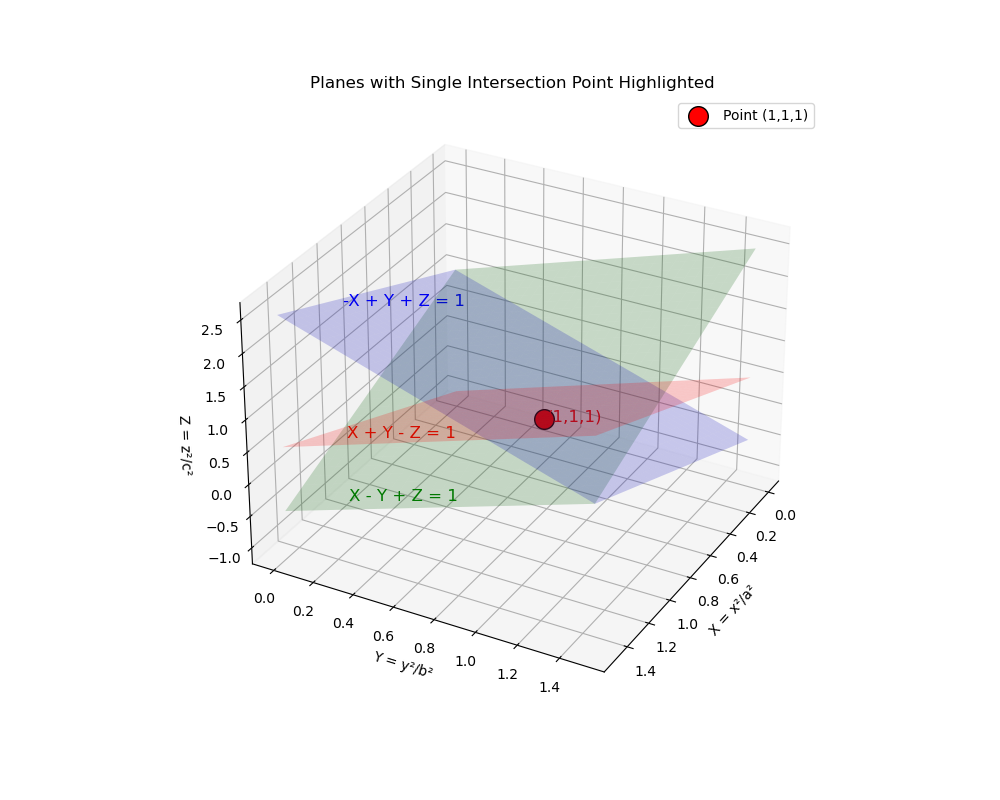
\includegraphics[width=0.55\linewidth]{figs/fig1.png}
    \caption{}
    \label{fig:placeholder}
\end{figure}

\end{document}










